\documentclass[border=10pt]{standalone}
\usepackage{tikz}
\usetikzlibrary{arrows.meta, positioning}

\begin{document}
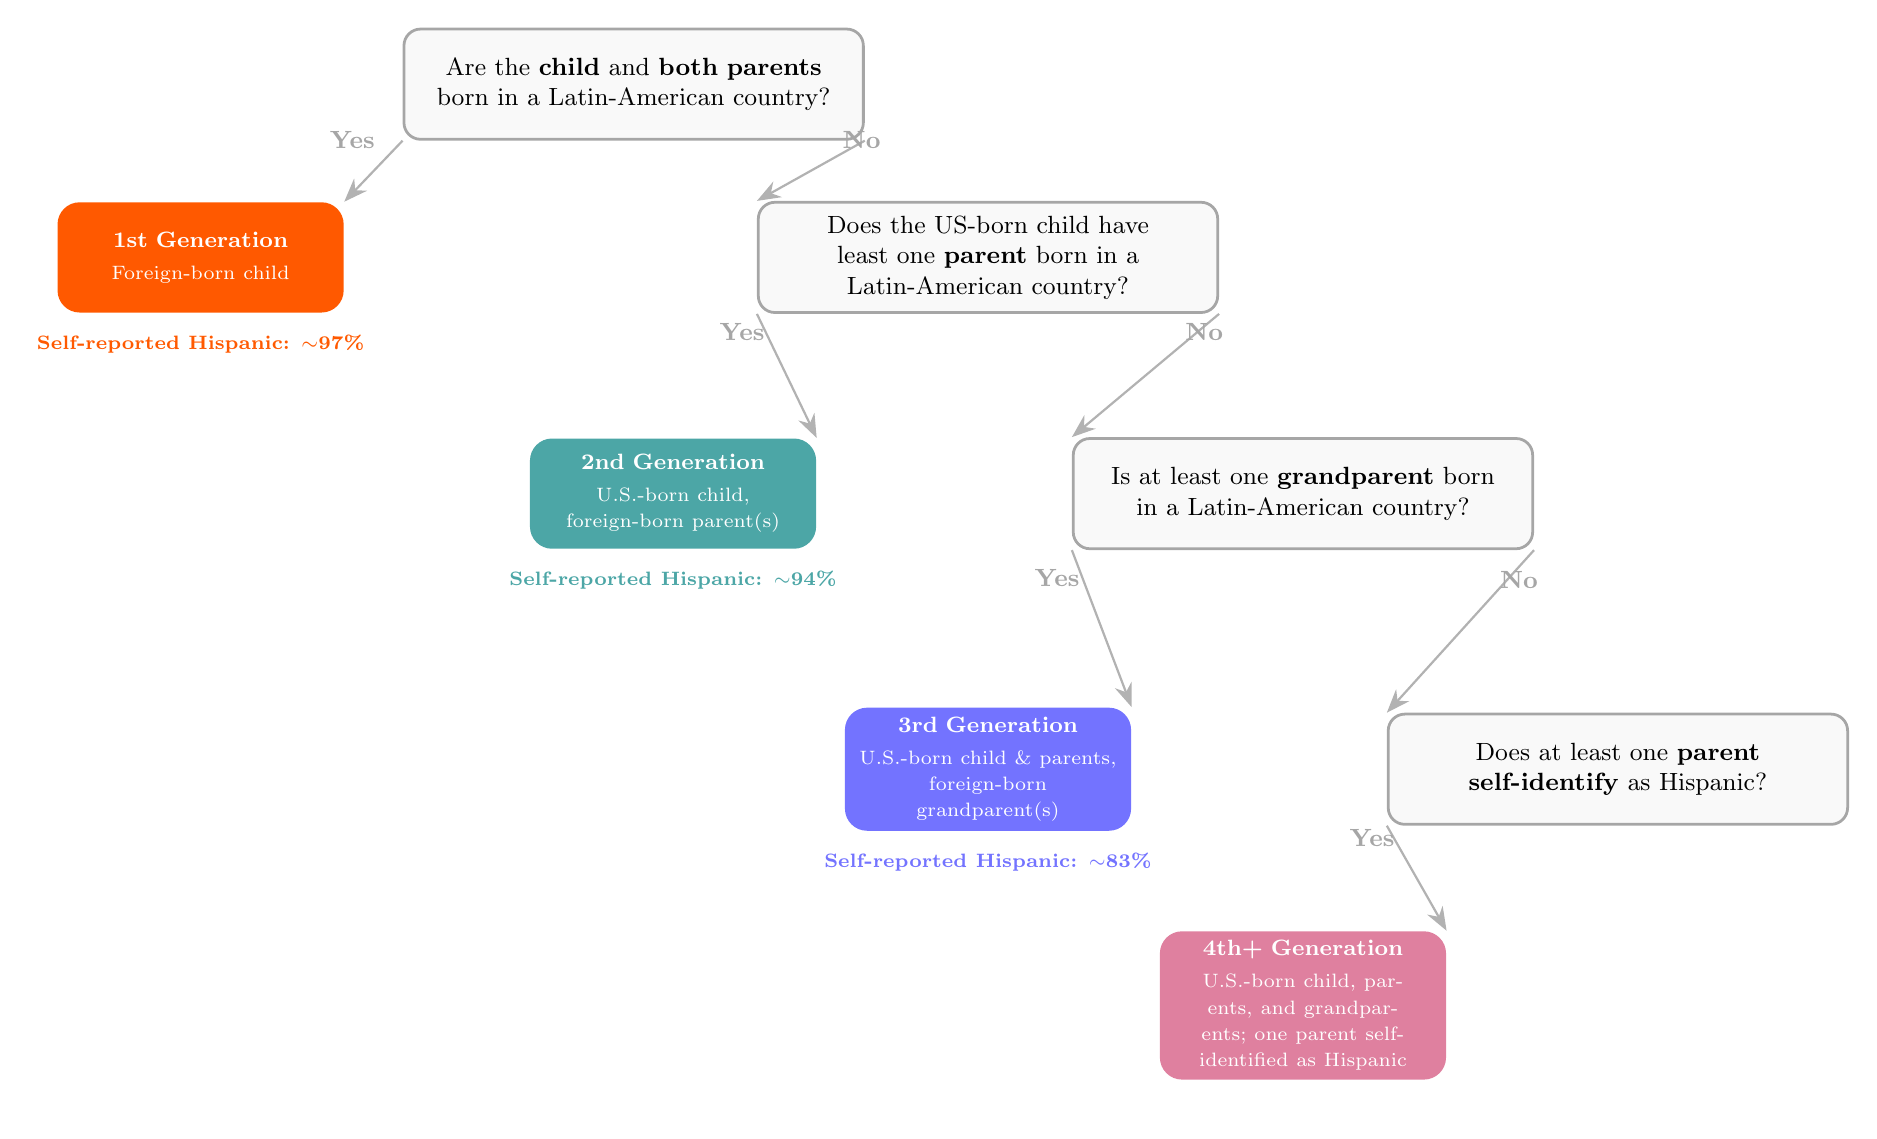
\begin{tikzpicture}[
  qbox/.style={rectangle, rounded corners=6pt, draw=gray!70, line width=1pt,
    minimum width=5.8cm, minimum height=1.4cm, text centered, text width=5.6cm,
    font=\small, fill=gray!5},
  genbox/.style={rectangle, rounded corners=8pt, draw=none,
    minimum width=3.6cm, minimum height=1.4cm, text centered, text width=3.4cm,
    font=\footnotesize, text=white},
  yesno/.style={font=\small\bfseries, text=gray!70},
  arr/.style={-{Stealth[length=3mm]}, thick, gray!60}
]
% === Level 0: Top question (child's own birthplace) ===
\node[qbox] (q1) at (0,0) {Are the \textbf{child} and \textbf{both parents} born in a Latin-American country?};
% === Level 1: Yes → 1st Gen ===
\node[genbox, fill=orange!70!red] (gen1) at (-5.5,-2.2)
  {\textbf{1st Generation}\\[2pt] {\scriptsize Foreign-born child}};
% === Level 1: No → next question (parents' birthplace) ===
\node[qbox] (q2) at (4.5,-2.2) {Does the US-born child have least one \textbf{parent} born in a Latin-American country?};
% === Level 2: Yes → 2nd Gen ===
\node[genbox, fill=teal!70] (gen2) at (0.5,-5.2)
  {\textbf{2nd Generation}\\[2pt] {\scriptsize U.S.-born child,}\\{\scriptsize foreign-born parent(s)}};
% === Level 2: No → next question (grandparents' birthplace) ===
\node[qbox] (q3) at (8.5,-5.2) {Is at least one \textbf{grandparent} born in a Latin-American country?};
% === Level 3: Yes → 3rd Gen ===
\node[genbox, fill=blue!55] (gen3) at (4.5,-8.7)
  {\textbf{3rd Generation}\\[2pt] {\scriptsize U.S.-born child \& parents,}\\{\scriptsize foreign-born grandparent(s)}};
% === Level 3: No → next question (parental self-ID) ===
\node[qbox] (q4) at (12.5,-8.7) {Does at least one \textbf{parent self-identify} as Hispanic?};
% === Level 4: Yes → 4th+ Gen ===
\node[genbox, fill=purple!50] (gen4) at (8.5,-11.7)
  {\textbf{4th+ Generation}\\[2pt] {\scriptsize U.S.-born child, parents, and grandparents; one parent self-identified as Hispanic}};
% === Arrows with Yes/No labels ===
\draw[arr] (q1.south west) -- node[yesno, above left, pos=0.3] {Yes} (gen1.north east);
\draw[arr] (q1.south east) -- node[yesno, above right, pos=0.3] {No} (q2.north west);
\draw[arr] (q2.south west) -- node[yesno, above left, pos=0.3] {Yes} (gen2.north east);
\draw[arr] (q2.south east) -- node[yesno, above right, pos=0.3] {No} (q3.north west);
\draw[arr] (q3.south west) -- node[yesno, above left, pos=0.3] {Yes} (gen3.north east);
\draw[arr] (q3.south east) -- node[yesno, above right, pos=0.3] {No} (q4.north west);
\draw[arr] (q4.south west) -- node[yesno, above left, pos=0.3] {Yes} (gen4.north east);
% === Self-ID rate annotations ===
\node[font=\scriptsize\bfseries, text=orange!70!red, below=0.15cm of gen1] {Self-reported Hispanic: $\sim$97\%};
\node[font=\scriptsize\bfseries, text=teal!70, below=0.15cm of gen2] {Self-reported Hispanic: $\sim$94\%};
\node[font=\scriptsize\bfseries, text=blue!55, below=0.15cm of gen3] {Self-reported Hispanic: $\sim$83\%};
\node[font=\scriptsize\bfseries, text=purple!50, below=0.15cm of gen4] {};
\end{tikzpicture}
\end{document}
